\documentclass{report}

\usepackage{amsmath}
\usepackage{amssymb}
\usepackage{siunitx}

\usepackage{xcolor}
\usepackage{tikz}
\usetikzlibrary{intersections, calc,through,backgrounds}

\usepackage{titlesec}
\usepackage[skins]{tcolorbox}

% colors
%%%%%%%%%%%%%%%%%%%%%%%%%%%%%%%%%%%%%%%%%%%%%%%%%%%%%%%%%%
\definecolor{i}{HTML}{FF0000}
\definecolor{j}{HTML}{00BB00}
\definecolor{k}{HTML}{0000FF}

%vega https://vega.github.io/vega/docs/schemes/#category10
\definecolor{1}{HTML}{1F77B4}
\definecolor{2}{HTML}{FF7F0E}
\definecolor{3}{HTML}{2CA02C}
\definecolor{4}{HTML}{D62728}
\definecolor{5}{HTML}{9467BD}
\definecolor{6}{HTML}{8C564B}
\definecolor{7}{HTML}{E377C2}
\definecolor{8}{HTML}{7F7F7F}
\definecolor{9}{HTML}{BCBD22}
\definecolor{10}{HTML}{17BECF}

\definecolor{problem}{HTML}{FFFCAB}
\definecolor{problem_frame}{HTML}{BBCC00}
%%%%%%%%%%%%%%%%%%%%%%%%%%%%%%%%%%%%%%%%%%%%%%%%%%%%%%%%%%

\newcommand{\bi}{\vec{i}}
\newcommand{\bj}{\vec{j}}
\newcommand{\bk}{\vec{k}}

%--------------------------------------------------

%define a new environment for problem statements
\newsavebox{\selvestebox}
\newenvironment{colbox}[1]
  {\newcommand\colboxcolor{#1}%
   \begin{lrbox}{\selvestebox}%
   \begin{minipage}{\dimexpr\columnwidth-2\fboxsep\relax}}
  {\end{minipage}\end{lrbox}%
   \begin{center}
   \fcolorbox{problem!50!black}{\colboxcolor}{\usebox{\selvestebox}}
   \end{center}}
   
\newcommand{\problem}[1]{\begin{colbox}{problem}#1\end{colbox}}

\newcommand{\trynewcommand[2]}%
{\@ifundefined{#1}{%
    \newcommand{#1}{#2}
 }{%
    \renewcommand{#1}{#2}
 }
}

\title{\textsc{Problem Set 1}\\Vectors and Matrices}
\begin{document}

\maketitle

\documentclass[main.tex]{subfiles}
\begin{document}

\section{Vectors}

\subsection*{1A-1}
\problem{Find the magnitude and direction of the vectors}

\subsubsection*{a)}
\problem{$\vec{i} + \vec{j} + \vec{k}$}

        \begin{align*}
            &= <1, 0, 0> + <0,1,0> + <0,0,1>\\
            &= <1,1,1>
        \end{align*}

        $\text{dir} \ \vec{A} = \frac{\vec{A}}{|\vec{A}|}$

        \begin{align*}
            &= \frac{<1,1,1>}{\sqrt{3}}\\
            &= <\frac{1}{\sqrt{3}}, \frac{1}{\sqrt{3}},\frac{1}{\sqrt{3}}>
        \end{align*}

\subsubsection*{b)}
\problem{$2\vec{i} - \vec{j} + 2\vec{k}$}

    \begin{align*}
        &= <2, 0, 0> - <0,1,0> + <0,0,2>\\
        &= <2,-1,2>\\
        &= \frac{<2,-1,2>}{\sqrt{2^2 + 1 + 2^2}}\\
        &= \frac{<2,-1,2>}{\sqrt{4 + 1 + 4}}\\
        &= \frac{<2,-1,2>}{\sqrt{9}}\\
        &= \frac{<2,-1,2>}{3}\\
        &= <\frac{2}{3}, -\frac{1}{3},\frac{2}{3}>
    \end{align*}


\subsubsection*{c)}
\problem{$3\vec{i} - 6\vec{j} + 2\vec{k}$}

    \begin{align*}
        &= <3, 0, 0> - <0,6,0> + <0,0,2>\\
        &= <3,-6,2>\\
        &= \frac{<3,-6,2>}{\sqrt{3^2 + -6^2 + 2^2}}\\
        &= \frac{<3,-6,2>}{\sqrt{9 + -36 + 4}}\\
        &= \frac{<3,-6,2>}{\sqrt{-23}}\\
        &= <\frac{3}{\sqrt{-23}}, -\frac{6}{\sqrt{-23}},\frac{2}{\sqrt{-23}}>
    \end{align*}

\subsection*{1A-2}
\problem{For what value(s) of $c$ will
$\frac{1}{5} \vec{i} - \frac{1}{5} \vec{j} +c \vec{k}$
be a unit vector?}

A unit vector $\vec{v}$ has $|\vec{v}| = 1$.
Thus for the vector $\vec{v}$ with components $<a, b, c>$,
$\sqrt{a^2 + b^2 + c^2} = 1$.

\begin{align*}
 c &= 1 - (a^2 + b^2)\\
  &= 1 - (\frac{1}{5}^2 + \frac{1}{5}^2)\\
  &= 1 - 2(\frac{1}{5}^2)\\
  &= 1 - (\frac{2}{25})\\
  &= \frac{23}{25}
\end{align*}



\subsection*{1A-3}

\subsubsection*{a)}
    \problem{If $P = (1,3,-1)$ and $Q = (0,1,1)$, find $\vec{A} = PQ$,
    $|\vec{A}|$ and $\text{dir}\ \vec{A}$.\\
    (The previous notation impiles $P$ and $Q$ are points, and $A$ is a vector joining them)}

    \begin{align*}
    \vec{A} &= P - Q \\
    &= (1,3,-1) - (0,1,1) \\
    &= <1,2,-2> \\
    \\
    |\vec{A}| &= \sqrt{1^2 + 2^2 + (-2)^2}\\
    &=\sqrt{1+4+4}\\
    &=\sqrt{9}\\
    &=3\\
    \\
    \text{dir} \ \vec{A} &= \frac{\vec{A}}{|\vec{A}|}\\
    &= \frac{1}{3} <1,2,-2>\\
    &= <\frac{1}{3},\frac{2}{3},\frac{-2}{3}>\\
    \end{align*}



\subsubsection*{b)}
    A vector $\vec{A}$ has magnitude 6 and
    direction $(\bi + 2\bj - 2\bk)/3$. If it's tail is at $(-2, 0 , 1)$,
    where is it's head?

    Let $A_t$ and $A_h$ represent the tip and the tail of the vector
    $\vec{A}$, respectivley.
    To get to the head of the vector all we need to do is start at the
    point $A_t$ and travel 6 units in the direction of $\vec{A}$.
    Which is to say:

    \begin{align*}
    A_h &= A_t + \vec{A}\\
    &= (-2,0,1) + 6(\bi + 2\bj - 2\bk)/3\\
    &= (-2,0,1) + 2(\bi + 2\bj - 2\bk)\\
    &= (-2,0,1) + <2,4, -4>\\
    &= (0,4,-3)\\
    \end{align*}

\subsection*{1A-4}

\subsubsection*{a)}
\problem{Let $P$ and $Q$ be two points in space, and $X$ the mid point of
the line segment $PQ$. Let $O$ be an arbitrary fixed point; show that as
vectors, $OX = \frac{1}{2}(OP + OQ)$.}

We begin with the points $O, P, Q$. $X$ is at the mid point from $P$
to $Q$.

Now consider the vectors $\vec{OP}$, $\vec{OX}$, and $\vec{OQ}$.
Let $R$ be the point at $\vec{OP} + \vec{OQ}$

\begin{align*}
\vec{OX} &= \vec{OP} + \vec{PX} \\
\vec{PX} &= \frac{1}{2}\vec{PQ} \\
\\
\vec{OX} &= \vec{OQ} + \vec{QX}\\
\vec{QX} &= -\frac{1}{2}\vec{PQ} \\
\end{align*}


\subsubsection*{b)}
\problem{With the notation of part (a), assume that $X$ divides the line
segment $PQ$  in the ratio $r : s$, where $r + s =1$. Derive an expression
for $OX$ in terms of $OP$ and $OQ$.}

    Consider first an expression for the vector $\vec{OX}$.
    We start at $O$, move to $P$, then from $P$ go to $X$,
    thus $\vec{OX} = \vec{OP} + \vec{PX}$.
    We know that from $P$ to $X$ we need to travel a fraction of the
    distance from $P$ to $Q$. Specifically, $\vec{PX} = r\vec{PQ}$.
    Thus $\vec{OX} = \vec{OP} + r\vec{PQ}$.

    We also can formulate an expression for $\vec{PQ}$ in terms
    of the points $O$, $P$, and $Q$. $\vec{PQ} = \vec{OQ} - \vec{OP}$


    \begin{align*}
    \therefore\\
        \vec{OX} &= \vec{OP} + r(\vec{OQ} - \vec{OP})\\
        &= \vec{OP} + r\vec{OQ} - r\vec{OP})\\
        &= r\vec{OQ} - (r-1)\vec{OP})\\
        &= r\vec{OQ} + (1-r)\vec{OP})\\
        \\
        s = 1 - r\\
        \therefore\\
        \vec{OX} = r\vec{OQ} + s\vec{OP}
    \end{align*}

\subsection*{1A-6}
\problem{A small plane wishes to fly due north at 200 mph (as seen from
the ground), in a wind blowing from the north east at 50 mph. Tell with
what vector velocity in the air it should travel (give the $i\ j$-
components).}

Lets say that due north is the $j$ direction, namely $<0,1>$,
because that lines up with the image I have for the y-axis, and
thus, east is in the direction of $i$, $<1,0>$.
Our target is a vector $T = <0, 200> = (0\bi + 200\bj)$.
The windspeed, $|\vec{W})|$ is 50 mph, and has a direction $\hat{\vec
{W}} = \frac{1}{\sqrt{2}}(i + j)$
Thus our heading velocity $\vec{V}$ ought to be $\vec{T} - \vec{W}$

\begin{align}
\vec{V} &= \vec{T} - \vec{W}\\
&= 200\bj - \frac{50}{\sqrt{2}}(i+j)\\
&= (- \frac{50}{\sqrt{2}}i + (200  - \frac{50}{\sqrt{2}}) \bj)\\
\therefore \vec{V} &\approx (- 35.4 \bi + 164.6 \bj)\ \text{mph}
\end{align}



\subsection*{1A-7}

\problem{Let $\vec{A} = a\bi + b\bj$ be a plane vector; find in terms of $a$
and $b$ the vectors $\vec{A}'$ and $\vec{A}''$ resulting from
rotating $\vec{A}$ by $\ang{90}$ a) clockwise b) counterclockwise.

(Hint: make $\vec{A}$ the diagonal of a rectangle with sides on the $
x$ and $y$-axes, and rotate the whole rectangle.)}

\subsubsection*{a) / b)}
\problem{rotating $\vec{A}$ by $\ang{90}$ clockwise and counterclockwise}

\begin{align*}
\vec{A} &= a\bi + b\bj\\
&= a<1,0> + b<0,1>\\
\end{align*}

\begin{align*}
\vec{A'} &= a<0,-1> + b <1,0>\\
&= b\bi -a\bj\\
\end{align*}\\

\begin{align*}
\vec{A''} &= a<0,1> + b <-1,0>\\
&= - b \bi + a\bj\\
\end{align*}



Consider the vector {\color{1}$\vec{A}$},
composed of {\color{2}$a\vec{i}$}$ +
${\color{3}$b\vec{j}$}.

$\vec{A}'$ is the vector resulting from rotating {\color{1}$\vec{A}$} by $\ang{90}$


Just like $\vec{A}$, $\vec{A}'$ is composed of a linear combination
of $\bi$ and $\bj$.
We can write $\vec{A}' = u\bi + v\bj$, where $u$ and $v$ are scalars.

We also know that $|\vec{A}'| = |\vec{A}| = 1$, and because $\vec{A}'
$ is $\ang{90}$ to $\vec{A}$ we know that $\vec{A} \cdot \vec{A}' = 0$
(Review the problems on dot products if that isnt immediatly obvious.)


So from above, we also deduce the following,

\begin{align*}
\sqrt{u^2 + v^2} &= 1\\
u^2 + v^2 &= 1^2\\
u^2 &= 1 - v^2\\
u &= \sqrt{1 - v^2}\\
\end{align*}

Though, it isn't clear to what extent that helps me...

Lets look at the solutions to $\vec{A} \cdot \vec{A}' = 0$ for a
moment. Since $\vec{A} = a\bi + b\bj$ we can substitute $a$ and $b$
for $A_1$ and $A_2$ respectivley.

\begin{align*}
\vec{A} \cdot \vec{A}' &= {A_1}{A'}_1 + {A_2}{A'}_2 = 0\\
\text{becomes}\\
&= a{A'}_1 + b{A'}_2\\
\text{and so}\\
a{A'}_1 &= - b{A'}_2
\end{align*}

We also know that $\vec{A}' = u\bi + v\bj$, and so we can rewrite
the above expression as
\begin{equation*}
au = - bv
\end{equation*}

rearranging we get
\begin{equation*}
\frac{a}{b} = - \frac{v}{u}
\end{equation*}

Looking back, we know that the lengths of the two vectors are the
same, so we have

\begin{align*}
\sqrt{a^2 + b^2} &= \sqrt{v^2 + u^2}\\
a^2 + b^2 &= v^2 + u^2\\
\end{align*}


rearanging to get $a$ by itself in both cases
\begin{align*}
a &= -\frac{bv}{u}\\
a^2 &= u^2 + v^2 - b^2
\end{align*}

and now substituting the equations into each other

\begin{align*}
{-\frac{bv}{u}}^2 &= u^2 + v^2 -b^2\\
-{bv}^2 &= u^4 + u^2v^2 -u^2b^2\\
b^2v^2 &= u^4 + u^2v^2 -u^2b^2\\
0 &= u^4 + u^2v^2 -u^2b^2 - b^2v^2\\
&= u^4 + u^2v^2 - b^2(u^2 + v^2)\\
&= u^2(u^2 + v^2) - b^2(u^2 + v^2)\\
b^2(u^2 + v^2) &= u^2(u^2 + v^2) \\
b^2 &= u^2 \\
b &= \pm u
\end{align*}


Now we have $b$ in terms of $u$ we can use this to get $a$ in terms
of $v$

\begin{align*}
a &= -\frac{bv}{u}\\
a &= \begin{cases}
      -\frac{uv}{u} & b= u \\
      \frac{uv}{u} & b= -u
   \end{cases}\\
a &= \begin{cases}
      -v & b= u \\
      v & b= -u
   \end{cases}
\end{align*}

So finally we can write $\vec{A}' = b\bi - a\bj$, and $\vec{A}'' = -b
\bi + a\bj$


\subsubsection*{c)}
Let $\bi' =(3\bi +4\bj)/5$. Show that $\bi'$
is a unit vector, and use the first part of the exercise to find a vector $
\bj'$ such that $\bi'$ , $\bj'$ forms a right-handed coordinate system.

In a right hand coordinate system the angle $\angle\bi\bj = \ang{-90}$.
Thus if $\bi'$ is substituted for $\vec{A}''$ in the above example, $
\bj'$ becomes $-b\bi + a\bj$.
In turn this is $\bj' = (-4\bi + 3\bj)/5$.

\subsection*{1A-8}

The direction (see definition above) of a space vector is in
engineering practice often given by its direction cosines. To
describe these, let $\vec{A} = a\bi + b\bj + c\bk$ be a space
vector, represented as an origin vector, and let $\alpha$, $\beta$,
and $\gamma$ be the three angles ($\leq\pi$) that $\vec{A}$ makes
respectively with $\bi$, $\bj$, and $\bk$.

\subsubsection*{a)}
\problem{Show that
$\text{dir}\ \vec{A} = \cos\alpha\bi + \cos\beta\bj + \cos\gamma\bk$ .
(The three coefficients are called the direction cosines of $\vec{A}$.)}

\begin{equation*}
\vec{A} = a\bi + b\bj +c\bk
\end{equation*}

Notice that the components $a$ and $b$ define the angle between $\vec
{A}$ and $\bk$

Above I have sketched out a representation on $\vec{A}$ in relation
to {\color{i}$\bi$}, {\color{j}$\bj$}, and {\color{k}$\bk$}.
The longer gray vector shows the projection of $\vec{A}$ onto the
plane spaned by {\color{i}$\bi$}{\color{j}$\bj$}.
Focusing our attention just to the last component, we can see that
the angle from {\color{k}$\bk$} to $\vec{A}$
is defined by the triangle it makes with the projection of $\vec{A}$
onto {\color{i}$\bi$}{\color{j}$\bj$}.

The angle $\gamma$, which is the angle from {\color{k}$\bk$} to $\vec{A}$,
can be determined from the trig relationship
\begin{equation*}
\cos{\gamma} = \frac{c}{|\vec{A}|}
\end{equation*}

Similarly the other angles are thus:

\begin{equation*}
\cos{\alpha} = \frac{a}{|\vec{A}|}\\
\cos{\beta} = \frac{b}{|\vec{A}|}
\end{equation*}

Finally the direction of $\vec{A} = \frac{\vec{A}}{|\vec{A}|}$.
Therefore

\subsubsection*{b)}
\problem{Express the direction cosines of $\vec{A}$ in terms of
$a$,$b$,$c$; find the direction cosines of the vector $-\bi +2\bj +2\bk$.}

\subsubsection*{c)}
\problem{Prove that three numbers $t$,$u$,$v$ are the direction cosines of a
vector in space if and only if they satisfy $t2+ u2+ v2=1$.}


\subsection*{1A-9}
\problem{Prove using vector methods (without components) that the line
segment joining the midpoints of two sides of a triangle is parallel
to the third side and half its length. (Call the two sides $\vec{A}$
and $\vec{B}$.)}

Take the triangle formed by the vectors $\vec{A}$, $\vec{B}$, and $
\vec{C}$, where
\begin{equation*}
\vec{A} + \vec{B} = \vec{C}
\end{equation*}

The midpoints sides $\vec{A}$ and $\vec{B}$ are the vectors
$\frac{1}{2}\vec{A}$, and $\frac{1}{2}\vec{B}$ respectivley.
The line segment joining these points can be expressed as a vector,

\begin{equation*}
\frac{1}{2}\vec{A} + \frac{1}{2}\vec{B}
\end{equation*}

This is the same as
\begin{equation*}
\frac{1}{2} (\vec{A} + \vec{B})
\end{equation*}

And because we know that $\vec{A} + \vec{B} = \vec{C}$, we therefore
have
\begin{equation*}
\frac{1}{2} (\vec{A} + \vec{B}) =  \frac{1}{2} \vec{C}
\end{equation*}


Thus the line joining the midpoints of two sides of a triangle are
parrallel to, and half the length of the third side


\subsection*{1A-10}
\problem{Prove using vector methods (without components) that the
midpoints of the sides of a space quadrilateral form a parallelogram.}

Lets take the points $O$, $P$, $Q$, and $R$ as the verticies of a
quadrilateral, as illustrated below.

\begin{figure}[!h]
\centering
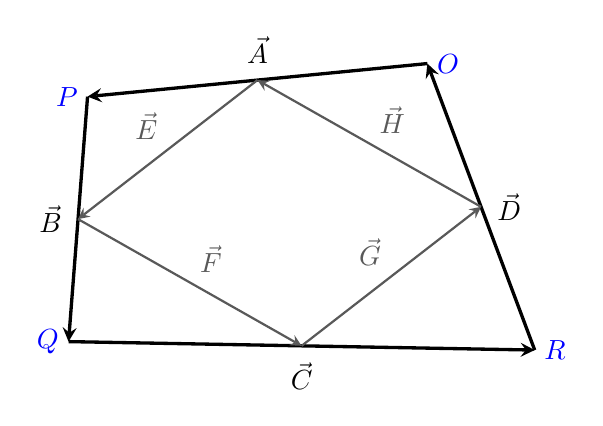
\begin{tikzpicture}
    [Vector qd/.style={->, very thick, color=black},
     Vector pg/.style={->, thick, color=black!65},
    >=stealth
    ]
%declare points OPQR at random locations
\coordinate[label=right:\textcolor{blue}{$O$}] (O) at ($(0,0) + (rand, rand)$);
\coordinate[label=left:\textcolor{blue}{$P$}] (P) at ($(-5,0) + (rand, rand)$);
\coordinate[label=left:\textcolor{blue}{$Q$}] (Q) at ($(-5,-3) + (rand, rand)$);
\coordinate[label=right:\textcolor{blue}{$R$}] (R) at ($(0,-3) + (rand, rand)$);

\coordinate (S) at ($(O)!0.5!(P)$);
\coordinate (T) at ($(P)!0.5!(Q)$);
\coordinate (U) at ($(Q)!0.5!(R)$);
\coordinate (V) at ($(R)!0.5!(O)$);

\draw[Vector qd, name=A]  (O) -- node[above=2pt]{$\vec{A}$} (P);
\draw[Vector qd, name=B]  (P) -- node[left=2pt]{$\vec{B}$} (Q);
\draw[Vector qd, name=C]  (Q) -- node[below=2pt]{$\vec{C}$} (R);
\draw[Vector qd, name=D]  (R) -- node[right=2pt]{$\vec{D}$} (O);

\draw[Vector pg]  (S) -- node[above left]{$\vec{E}$} (T);
\draw[Vector pg]  (T) -- node[above right]{$\vec{F}$} (U);
\draw[Vector pg]  (U) -- node[above left]{$\vec{G}$} (V);
\draw[Vector pg]  (V) -- node[above right]{$\vec{H}$} (S);

\end{tikzpicture}
\end{figure}

Consider the vectors that run along the edges, pointing in the counterclockwise
direction, labelled $\vec{A}$, $\vec{B}$, $\vec{C}$, and $\vec{D}$.
In particular,
\begin{align*}
\vec{A} = \vec{OP} = P - O\hspace{5em}
\vec{B} = \vec{PQ} = Q - P\\
\vec{C} = \vec{QR} = R - Q\hspace{5em}
\vec{D} = \vec{RO} = O - R.
\end{align*}

Let $\vec{E}$ be vector connecting the midpoints of $OP$ and $PQ$.
Which, in terms of $\vec{A}$ and $\vec{B}$, becomes
\[\vec{E} = \frac{1}{2}(\vec{A} + \vec{B})\].
Similarly, the vector connecting the midpoints of $QR$ and $RO$, which
we will denote $\vec{G}$, can be expressed as
\[\vec{G} = \frac{1}{2}(\vec{C} + \vec{D})\].

Now if we expand out $\vec{A} + \vec{B}$, we get
\begin{align*}
\vec{A} + \vec{B} &= \vec{OP} + \vec{PQ}\\
                  &= P - O + Q - P\\
                  &=  Q - O \\
                  &=  \vec{OQ} \\
\end{align*}

Meanwhile, expanding $\vec{C} + \vec{D}$ yeilds
\begin{align*}
\vec{C} + \vec{D} &= \vec{QR} + \vec{RO}\\
                  &= R - Q + O - R\\
                  &=  O - Q \\
                  &=  \vec{QO} \\
                  &=  -\vec{OQ}. \\
\end{align*}

Thus $\vec{A} + \vec{B} = -(\vec{C} + \vec{D})$.
Which is to say the vectors $\vec{E}$ and $\vec{G}$ run anti-parrallel
and have the same magnitude. By the same process we can deduce
$\vec{B}+\vec{C} = -(\vec{D}+\vec{A})$.
Which in turn means that the vectors $\vec{H}$ and $\vec{F}$ also run
anti-parallel  and have the same magnitude.

Therefore we the shape formed by connecting the midpoints of a
quadrilateral is a parallelogram.



\subsection*{1A-11}

\problem{Prove using vector methods (without components) that the
 diagonals of a parallelogram bisect each other. \\
(One way: let $\vec{X}$ and $\vec{Y}$ be the midpoints of the two
diagonals; show $\vec{X} = \vec{Y}$.)}

Let's consider the parallelogram $OPQR$, where $O$, $P$, $Q$, and $R$
represent the coordinates of the verticies, running in counterclockwise
order.

\begin{figure}[!h]
\centering
\begin{tikzpicture}
% layout some coordinates for a parallelogram
\coordinate[label=\textcolor{blue}{$O$}] (O) at ($(0,0)$);
\coordinate[label=\textcolor{blue}{$P$}] (P) at ($(-3, 1)$);
\coordinate[label=below:\textcolor{blue}{$Q$}] (Q) at ($(-2, -2)$);
\coordinate[label=below:\textcolor{blue}{$R$}] (R) at ($(1, -3)$);

\draw[thin] (O) -- (P);
\draw[thin] (P) -- (Q);
\draw[thin] (Q) -- (R);
\draw[thin] (R) -- (O);

\end{tikzpicture}
\caption{the parallelogram $OPQR$}
\end{figure}

Notice that the parallelogram can be represented by the span of two vectors,
$\vec{A}$ and $\vec{B}$.
In fact if we say that the point $O$ is the origin, then each edge of $OPQR$
can be specified in terms of $\vec{A}$ and $\vec{B}$.


\begin{tcolorbox}[boxsep=.5mm, boxrule=.1pt]
\textit{ie.}\\
\begin{align*}
\vec{A} = P - O \hspace{5em}
Q-R = P-O = \vec{A}\\
\vec{B} = R - O\hspace{5em}
Q-P = R-O = \vec{B}
\end{align*}
\tcblower
Conversly we can think of each point in terms of the vector combination we need to
add to $O$ in order to get to that point.
\begin{align*}
P = \vec{A} \hspace{5em}
R = \vec{B} \hspace{5em}
Q = \vec{A} + \vec{B}
\end{align*}
\end{tcolorbox}

\begin{figure}[!h]
\centering
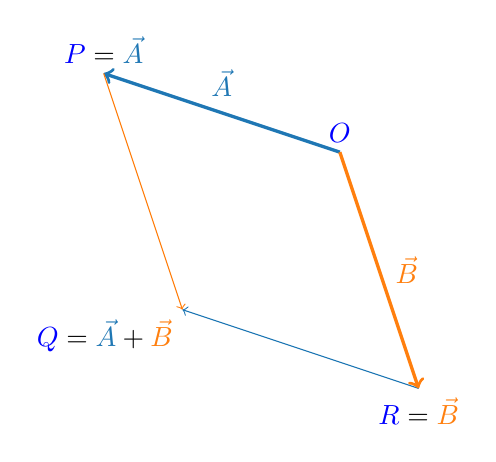
\begin{tikzpicture}
% layout some coordinates for a parallelogram
\coordinate[label=\textcolor{blue}{$O$}] (O) at ($(0,0)$);
\coordinate[label={${\color{blue}P} = \color{1}\vec{A}$}] (P) at ($(-3, 1)$);
\coordinate[label=below left:%
{${\color{blue}Q} = {\color{1}\vec{A}} + {\color{2}\vec{B}}$}]%
 (Q) at ($(-2, -2)$);
\coordinate[label=below:{${\color{blue}R} = {\color{2}\vec{B}}$}] (R) at ($(1, -3)$);

\draw[->, color=1, very thick] (O) -- node[color=1, above=2pt]{$\vec{A}$} (P);
\draw[->, color=2, thin] (P) -- (Q);
\draw[<-, color=1, thin] (Q) -- (R);
\draw[<-, color=2, very thick] (R) --node[color=2, right=2pt]{$\vec{B}$} (O);

\end{tikzpicture}
\caption{the parallelogram $OPQR$ in terms of $\vec{A}$ and $\vec{B}$}
\end{figure}

Now let $\vec{U}$ and $\vec{V}$ be the vectors that run accross the diagonals,
such that $\vec{U} = \vec{A} + \vec{B}$ and $\vec{V} = \vec{A} - \vec{B}$.

\begin{figure}[!h]
\centering
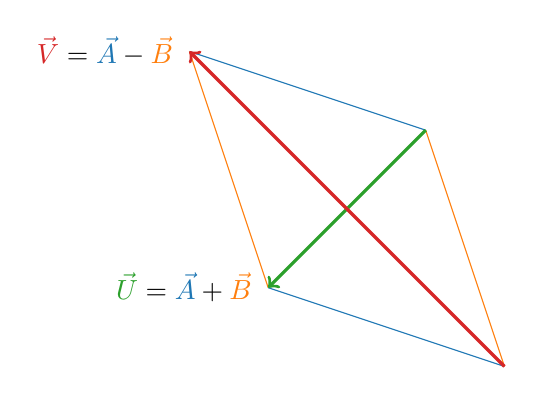
\begin{tikzpicture}
% layout some coordinates for a parallelogram
\coordinate (O) at ($(0,0)$);
\coordinate (P) at ($(-3, 1)$);
\coordinate (Q) at ($(-2, -2)$);
\coordinate (R) at ($(1, -3)$);

\draw[thin, color=1]  (O) -- (P);
\draw[thin, color=2]  (P) -- (Q);
\draw[thin, color=1]  (Q) -- (R);
\draw[thin, color=2]  (R) -- (O);

\draw[->, very thick, name=U, color=3]  (O) -- node[left=2pt, at end]{$\color{black}{\color{3}\vec{U}} =
                                                 {\color{1}\vec{A}}
                                                 + {\color{2}\vec{B}}$
                                                 } (Q);
\draw[->, very thick, name=V, color=4]  (R) -- node[left=2pt, at end]{$\color{black}{\color{4}\vec{V}} =
                {\color{1}\vec{A}} - {\color{2}\vec{B}}$
                } (P);

\end{tikzpicture}
\caption{the parallelogram $OPQR$ with diagonals illustrated as $\vec{U}$ and $\vec{V}$}
\end{figure}

If the two vectors were to bisect, we could find some pair of values,
$\{a,b\}$, such that \[ a\vec{U} = \vec{B} + b\vec{V}. \]
So now we solve for $a$ and $b$.
\begin{align*}
a\vec{U} &= \vec{B} + b\vec{V}\\
a\vec{U} &=  \vec{B} + b\vec{V},
\hspace{2em}\vec{U} = \vec{A}+\vec{B},
\hspace{2em}\vec{V} = \vec{A}-\vec{B}\\
a(\vec{A} + \vec{B}) &= \vec{B} + b(\vec{A}-\vec{B})\\
a(\vec{A} + \vec{B}) &= \vec{B} + b\vec{A}-b\vec{B}\\
a(\vec{A} + \vec{B}) &= (1-b)\vec{B} + b\vec{A}\\
\vec{A} + \vec{B} &= \frac{(1-b)\vec{B} + b\vec{A}}{a}\\
\vec{A} + \vec{B} &= \frac{(1-b)}{a}\vec{B} + \frac{b}{a}\vec{A}\\
\vec{A} + \vec{B} &= \frac{b}{a}\vec{A} + \frac{(1-b)}{a}\vec{B} \\
0 &= \frac{b}{a}\vec{A} -\vec{A} + \frac{(1-b)}{a}\vec{B}  -\vec{B}\\
0 &= (\frac{b}{a} - 1)\vec{A} + (\frac{(1-b)}{a} - 1)\vec{B}
\end{align*}

We know that $\vec{A} + \vec{B} \neq 0$. We also know that $\vec{A}$ and $\vec{B}$
point in two different directions, that is, they are linearly independant. If this
were not the case then our parallelogram would be squished onto a single line.
In other words, the only time that the tips of $\vec{A}$ and $\vec{B}$ intersect,
given place their tails start at the origin, is when the length of both vectors is $0$.

Therefore,
\[(\frac{b}{a} - 1) = (\frac{(1-b)}{a} - 1) = 0.\]
\begin{align*}
\frac{b}{a} - 1 &= 0\\
\frac{b}{a} &= 1\\
b &= a,
\end{align*}

and,
\begin{align*}
\frac{(1-b)}{a} - 1 &= 0\\
\frac{(1-a)}{a} - 1 &= 0\\
\frac{1}{a} - 1 &= 1\\
\frac{1}{a} &= 2\\
a &= \frac{1}{2}.
\end{align*}

So we find that the diagnoals intersect at their midpoints,
$\frac{1}{2}\vec{U} = \vec{B} + \frac{1}{2}\vec{V}$. This relationship
tells us that we travel halfway along $\vec{U}$ from $O$ we get to the same point
as we would if we started at $R$ and traveled halfway along $\vec{V}$.

\subsection*{1A-12*}
\problem{Label the four vertices of a parallelogram in counterclockwise order
 as $OPQR$. Prove that the line segment from $O$ to the midpoint of $PQ$
 intersects the diagonal $PR$ in a point $X$ that is $1/3$ of the way from $P$
 to $R$.

(Let $\vec{A} =OP$, and $\vec{B} =OR$; express everything in terms of
$\vec{A}$ and $\vec{B}$.)}

Take the parallelogram $OPQR$. Let $\vec{U}$ be the vector along the diagonal
$PR$, $\vec{V}$ be the vector along the other diagonal ($OQ$), and $\vec{W}$ be
the vector from $O$ to the midpoint of $PQ$. Also let $S$ be the midpoint of $PQ$.

Note that $\vec{U} = \vec{B}-\vec{A}$, \
and that $\vec{W} =\frac{1}{2}\vec{B} + \vec{A}$.


\begin{figure}[!h]
\centering
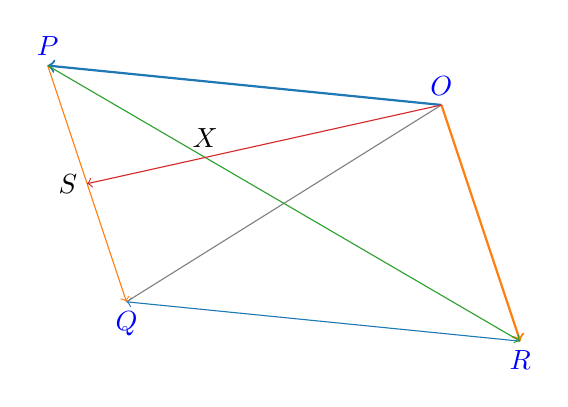
\begin{tikzpicture}
% layout some coordinates for a parallelogram
\coordinate[label=\textcolor{blue}{$O$}] (O) at ($(0,0)$);
\coordinate[label=\textcolor{blue}{$P$}] (P) at ($(-5, 0.5)$);
\coordinate[label=below:\textcolor{blue}{$Q$}] (Q) at ($(-4, -2.5)$);
\coordinate[label=below:\textcolor{blue}{$R$}] (R) at ($(1, -3)$);
\coordinate (mid) at ($(P)!0.5!(Q)$);

\draw[->, thick, color=1, name path=A] (O) -- (P);
\draw[->,thin, color=2, name path=B] (P) -- (Q);
\draw[->, thin, color=1]  (R) -- (Q);
\draw[->, color=2, thick] (O) -- (R);

\draw[thin, black!50] (O) -- (Q);
\draw[->, color=3, thick, name path=U, thin] (P) -- (R);
\draw[->, color=4, thick, name path=W, thin] (O) -- (mid);

%label intersection then place a coordinate there
\path[name intersections={of=U and W}];
\coordinate[label=above:$X$] (X) at (intersection-1);

\path[name intersections={of=B and W}];
\coordinate[label=left:$S$] (S) at (intersection-1);

\end{tikzpicture}
\caption{the parallelogram $OPQR$}


\end{figure}

Consider that the vector $\vec{W}$ is composed of the sum of the vectors
$\vec{OX}$ and $\vec{XS}$. Like wise, $\vec{U}$ can be expressed as the sum
of $\vec{RX}$ and $\vec{XP}$.
A more convenient way of expressing this is through the use of scalars. Thus,
\[\vec{W} = \vec{OX} +\vec{XS} = a\vec{W} + b\vec{W},\] and
\[\vec{U} = \vec{RX} +\vec{XP} = c\vec{U} + d\vec{U}.\]


Now, consider the triangles $PXS$ and $ORX$. The first of these is defined by the following,
\begin{align*}
{\color{2}PS} &= {\color{3}PX} + {\color{4}XS}\\
{\color{2}\frac{1}{2}\vec{B}} &= {\color{3}- d\vec{U}} + {\color{4}b\vec{W}}\\
{\color{2}\frac{1}{2}\vec{B}} &= {\color{4}b\vec{W}} - {\color{3}d\vec{U}}.\\
\end{align*}
While the larger triangle is defined as
\begin{align*}
{\color{2}OR} &= {\color{4}OX} + {\color{3}XR}\\
{\color{2}\vec{B}} &= {\color{4}a\vec{W}} + {\color{3}-c\vec{U}}\\
{\color{2}\vec{B}} &= {\color{4}a\vec{W}} - {\color{3}c\vec{U}}.\\
\end{align*}
Taking these two relationships together we get,
\[\vec{B} = a\vec{W} - c\vec{U} = 2(b\vec{W} - d\vec{U}),\]
Which we can rearrange to solve for $a$ and $c$
(after noticing that $b = 1-a$ and $d = 1-c$).
\begin{align*}
a\vec{W} - c\vec{U} &= 2(b\vec{W} - d\vec{U})\\
a\vec{W} - 2b\vec{W} &=  c\vec{U} - 2d\vec{U}\\
(a - 2b)\vec{W} &=  (c - 2d)\vec{U}\\
(a - 2(1-a))\vec{W} &=  (c - 2(1-c))\vec{U}\\
(a - 2 + 2a)\vec{W} &=  (c - 2 + 2c)\vec{U}\\
(3a - 2)\vec{W} &=  (3c - 2)\vec{U}
\end{align*}

At this point we can apply similar logic as we did in the previous example.
We know that $\vec{W}$ and $\vec{U}$ are linearly independant.
So there is no $x,y$ where $x\vec{W} = y\vec{U}$, except the case when $x=y=0$.
Therefore,
\begin{align*}
(3a - 2) &= (3c - 2) = 0\\
3a - 2 &= 0\\
3a &= 2\\
a &= c = \frac{2}{3}.\\
\end{align*}

So now we can say that $X$ is at $P + d\vec{RP}$.
 Which can be expressed in terms of $\vec{A}$ and $\vec{B}$ as
 $\vec{A} + d(\vec{B} - \vec{A})$. And because $d = 1-c$ we can
 finally write \[X = \vec{A} + \frac{1}{3}(\vec{B} - \vec{A})\]
 \[X = \frac{2\vec{A} + \vec{B}}{3}.\]


\subsection*{1A-13*}
\problem{
    \subsubsection*{a)} Take a triangle $PQR$ in the plane; prove that as
    vectors $\vec{PQ}+\vec{QR}+\vec{RP} = 0$.}

We start by considering the triangle $PQR$,
with it's edges defined by the vectors $\vec{A}$, $\vec{B}$, $\vec{C}$.

\tikz[scale=2] {
    \coordinate (P) at ($(0,1) + .5*(rand, rand)$);
    \coordinate (Q) at ($(1,0) + .5*(rand, rand)$);
    \coordinate (R) at ($(-1, 0) + .5*(rand, rand)$);
    \coordinate (O) at (barycentric cs:P=1,Q=1,R=1);
}

\begin{figure}[!h]
\centering
\begin{tikzpicture}
% layout some coordinates for a triangle

\begin{scope}[thick]
\draw[->] (P) -- node[midway, above] {$\vec{A}$}(Q);
\draw[->] (Q) -- node[midway, below] {$\vec{B}$}(R);
\draw[->] (R) -- node[midway, above] {$\vec{C}$}(P);
\end{scope}

\node at (O) {$O$};
\node at (P) [above=2pt]{$P$};
\node at (Q) [right=2pt]{$Q$};
\node at (R) [left=2pt]{$R$};


\end{tikzpicture}
\caption{the triangle $PQR$}
\end{figure}

Notice that if you start at $P$ and travel along each vector $\vec{A}$, $\vec{B}$,
and $\vec{C}$ you find yourself returning to point $P$. Also, notice that
\[\vec{A} + \vec{B} = -\vec{C}.\]
Thus,
\begin{align*}
\vec{A} + \vec{B} + \vec{C}\\ &= \vec{A} + \vec{B}  - (\vec{A} + \vec{B})\\
&= \mathbf{0}.
\end{align*}

\problem{\subsubsection*{b)}

    Continuing part a), let A be a vector the same length as $\vec{PQ}$, but
    perpendicular to it, and pointing outside the triangle. Using similar
    vectors $\vec{B}$ and $\vec{C}$ for the other two sides, prove that
    $\vec{A} + \vec{B} + \vec{C} = \mathbf{0}$.
    (This only takes one sentence, and no computation.)}

    \begin{figure}[!h]
    \centering
    \begin{tikzpicture}

        % 1. Coordinates of the line segment projection to O: E,F,G
        % 2. draw the vectors from O passing through relevant midpoint
        \foreach \proj/\tip/\tail/\vector in {E/P/Q/A, F/Q/R/B, G/R/P/C}{
            \coordinate (\proj) at ($(\tip)!(O)!(\tail)$);

            \draw[->, thick] let
                \p1 = ($(\tip)-(\tail)$)
            in
                (O)--++($(O)!sqrt(\x1*\x1+\y1*\y1)!(\proj)-(O)$);
        }

        % Draw triangle, and midpoint markers
        \draw [thin] (P) -- (Q) -- (R) -- cycle;

        % Labels: verticies
        \node at (O) [left=2pt]{$O$};
        \node at (P) [above right=2pt]{$P$};
        \node at (Q) [right=2pt]{$Q$};
        \node at (R) [left=2pt]{$R$};

        % Labels: midpoints
        \begin{scope}[black!40]
        \node at (E) [above=1.5em]{$E$};
        \node at (F) [below left=.5em]{$F$};
        \node at (G) [above=1.5em]{$G$};
        \end{scope}
    \end{tikzpicture}
    \caption{the triangle $PQR$ with vectors at centre}
    \end{figure}


\subsection*{1A-14*}
\problem{Generalize parts a) and b) of the previous exercise to a closed
polygon in the plane which doesn’t cross itself (i.e., one whose interior is a
single region); label its vertices $P_1$, $P_2$ ,$...$ ,$P_n$ as you walk
around it.}

\subsection*{1A-15*}
\problem{Let $P_1$ , $...$ ,$P_n$ be the vertices of a regular $n$-gon in the
 plane, and $O$ its center; show without computation or coordinates that
 $OP_1 + OP_2 + ... + OP_n = 0$,
a) if $n$ is even; b) if $n$ is odd.}


\end{document}


\end{document}
